
\documentclass[sigconf]{acmart}


\usepackage{booktabs} % For formal tables
\usepackage[ruled,vlined]{algorithm2e}
\usepackage{amsmath}
\usepackage{wrapfig} 
\usepackage{balance}
\usepackage{enumitem}
\usepackage{moresize}
\usepackage{subcaption}
\usepackage{epstopdf}
\usepackage{graphicx} 
%\usepackage{geometry}
\usepackage{marginnote}
\usepackage{color}

% \usepackage{pslatex}
\usepackage{multirow} 

\usepackage{enumitem}
\usepackage{bm}
\usepackage{balance}

\newcommand{\newtext}[1]{{\color{blue} #1}}
\newcommand{\margincomment}[1]{\marginnote{{[{\sf {\color{red}\scriptsize #1}}]}}}
\newcommand{\Margincomment}[1]{\marginnote{{[{\sf {\color{blue}\scriptsize #1}}]}}}


\definecolor{myGreen}{rgb}{0.31, 0.78, 0.47}
\definecolor{myRed}{rgb}{0.73, 0.31, 0.28}
\definecolor{myBlue}{rgb}{0, 0.44, 1}
\definecolor{myGrey}{rgb}{0.57, 0.64, 0.69}

\usepackage{array}
\newcommand{\PreserveBackslash}[1]{\let\temp=\\#1\let\\=\temp}
\newcolumntype{C}[1]{>{\PreserveBackslash\centering}p{#1}}
\newcolumntype{R}[1]{>{\PreserveBackslash\raggedleft}p{#1}}
\newcolumntype{L}[1]{>{\PreserveBackslash\raggedright}p{#1}}

%\newcommand\comment[1]{[\textcolor{red}{#1}]
\newcommand\Paragraph[1]{\vspace{0.02in}  \noindent \textbf{#1.}}
\newcommand\Paragraphq[1]{\vspace{0.02in}  \noindent \textbf{#1?}}
\newcommand\Paragraphno[1]{\vspace{0.02in}  \noindent \textbf{#1}}
\newcommand\Textcolor[2]{\hspace*{-3mm} \textcolor{#1}{#2} }

\newcommand{\shubham}[1]{\textcolor{myGreen}{#1}}
\newcommand{\manos}[1]{\textcolor{myRed}{#1}}
\newcommand{\subhadeep}[1]{\textcolor{myBlue}{#1}}


% \AtBeginDocument{%
%   \providecommand\BibTeX{{%
%     Bib\TeX}}}

% \setcopyright{acmcopyright}
% \copyrightyear{2018}
% \acmYear{2018}
% \acmDOI{XXXXXXX.XXXXXXX}

% \acmConference[Conference acronym 'XX]{Make sure to enter the correct
%   conference title from your rights confirmation emai}{June 03--05,
%   2018}{Woodstock, NY}
  
% \acmPrice{15.00}
% \acmISBN{978-1-4503-XXXX-X/18/06}


\begin{document}


\title{LSM Memory Profiling}

\author{****}
\affiliation{%
    \institution{}
    \country{}
}

\author{****}
\affiliation{%
    \institution{}
    \country{}
}

\author{****}
\affiliation{%
    \institution{}
    \country{}
}

% \author{Ben Trovato}
% \authornote{Both authors contributed equally to this research.}
% \email{trovato@corporation.com}
% \orcid{1234-5678-9012}
% \author{G.K.M. Tobin}
% \authornotemark[1]
% \email{webmaster@marysville-ohio.com}
% \affiliation{%
%   \institution{Institute for Clarity in Documentation}
%   \streetaddress{P.O. Box 1212}
%   \city{Dublin}
%   \state{Ohio}
%   \country{USA}
%   \postcode{43017-6221}
% }

% \author{Lars Th{\o}rv{\"a}ld}
% \affiliation{%
%   \institution{The Th{\o}rv{\"a}ld Group}
%   \streetaddress{1 Th{\o}rv{\"a}ld Circle}
%   \city{Hekla}
%   \country{Iceland}}
% \email{larst@affiliation.org}

% \author{Valerie B\'eranger}
% \affiliation{%
%   \institution{Inria Paris-Rocquencourt}
%   \city{Rocquencourt}
%   \country{France}
% }

% \author{Aparna Patel}
% \affiliation{%
%  \institution{Rajiv Gandhi University}
%  \streetaddress{Rono-Hills}
%  \city{Doimukh}
%  \state{Arunachal Pradesh}
%  \country{India}}

% \author{Huifen Chan}
% \affiliation{%
%   \institution{Tsinghua University}
%   \streetaddress{30 Shuangqing Rd}
%   \city{Haidian Qu}
%   \state{Beijing Shi}
%   \country{China}}

% \author{Charles Palmer}
% \affiliation{%
%   \institution{Palmer Research Laboratories}
%   \streetaddress{8600 Datapoint Drive}
%   \city{San Antonio}
%   \state{Texas}
%   \country{USA}
%   \postcode{78229}}
% \email{cpalmer@prl.com}

% \author{John Smith}
% \affiliation{%
%   \institution{The Th{\o}rv{\"a}ld Group}
%   \streetaddress{1 Th{\o}rv{\"a}ld Circle}
%   \city{Hekla}
%   \country{Iceland}}
% \email{jsmith@affiliation.org}

% \author{Julius P. Kumquat}
% \affiliation{%
%   \institution{The Kumquat Consortium}
%   \city{New York}
%   \country{USA}}
% \email{jpkumquat@consortium.net}


% \renewcommand{\shortauthors}{Trovato et al.}


\begin{abstract}
  In modern data systems, particularly for write-intensive workloads, log-structured merge (LSM) trees have become the most 
widely used technique. The idea of out-of-place updates, which logically 
invalidate keys that may exists on multiple levels, helps LSM-trees excel for write heavy workloads. However, current 
LSM-tree designs do not capitalize on the sort-merge operations performed for the range queries, which leads to carrying 
out almost the same amount of work for each range query, even when they are same or overlapping. This inefficiency can 
result in the wastage of CPU cycles and unnecessary I/O operations in worst-case scenarios due to presence of logically 
invalid keys. \cite{sarkar2021}  
\end{abstract}

% \keywords{datasets, neural networks, gaze detection, text tagging}



\maketitle

\section{Introduction}
\label{sec:intro}
This is the Introduction section.

\section{Background}
\label{sec:background}
This is the background section. 


\section{Problem}
\label{sec:design_space}
Here are the descriptions of all buffer implementations.
 
\section{Solution Name}
\label{sec:solution}
\input{4-solution}

% \section{Results}
% \label{sec:results}
% \input{5-analytical_results}

\section{Evaluation}
\label{sec:experimental_results}

\lipsum[1]

\subsection{Experimental Setup}
\lipsum[1]

\subsection{Footprint Profiling}
\lipsum[1]

\subsection{Performance Profiling}
\lipsum[1]

% \begin{figure}[h]
%   \centering
%   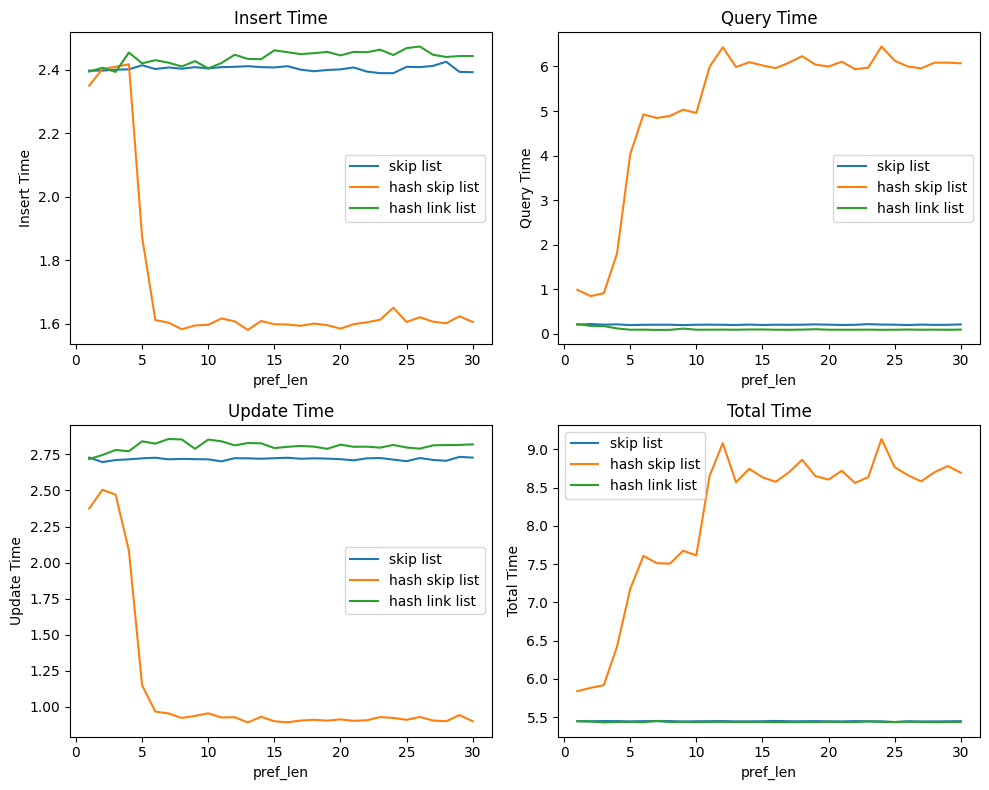
\includegraphics[width=0.5\linewidth]{Figures/trial_graph.png}
%   \caption{Placeholder Image}
%  \label{fig:placeholder}
% \end{figure}




\section{Related Work}
\label{sec:related_work}
\input{7-related_work}
 
\section{Conclusion}
\label{sec:conclusion}
LSM-based storage engines performs well for write intensive workloads. 
The performance and configuration of write buffers are always treated as a default setting in most of the storages.
The insights of workload and a better configuration of write buffer can improve the performance at the next level.
In this paper, we have benchmarked the performance of LSM-based storage engines with different memory buffer implementations and under different workload characteristics.
We experiment with four buffer implementations, namely, (i) \textit{vector}, (ii) \textit{skip-list}, (iii) \textit{hash skip-list}, and (iv) \textit{hash linked-list}, and for each implementation, we vary any design choices (such as bucket count and prefix length in a hash linked-list or hash skip-list).
We also explored the tunning knobs for the \textit{vector} that can save the write-stalls for resizing the buffer to accumulate the incoming writes.
The right configuration for the write buffer can improve the overall performance of the LSM-based storage engines. 
We plan to come up with more variant of the write buffer implementations and their performance benchmarking in the future.


\balance 
{
\input{biblio} 
} 

\end{document}
\endinput

